\section{Proposed Work}\label{section-proposed-work}
The iteration of the development could be reduce in two ways:
\begin{enumerate}
    \item Processing Debug/Unsigned BIOS in section \ref{subsection-processing-bios}
    \item Processing Firmware individually in section \ref{subsection-processing-firmware}
\end{enumerate}

\subsection{Processing Unsigned debug BIOS}\label{subsection-processing-bios}
Before Releasing the BIOS firmware for public use, those are signed for security and integrity purpose, however the debug BIOS which are used Pre-release to test and verify all the functional features until all the requirements are met.

Every \gls{soc} system which are under test known is \gls{sut} are configured in such a way that it supports debug BIOS. The proposed framework is designed to simulate the process of \gls{sut} in terms of processing BIOS binary similar to \gls{sut} performs it after flashing BIOS firmware on \gls{soc}. 


Processing the debug BIOS can be classified in to two ways:
\begin{enumerate}\label{cli-classification-proposed-work}
	\item Applying changes directly to the \gls{sut}
	\item Applying changes on to the BIOS binary
\end{enumerate}

At the high level the flow for both the above classification remains the same but will be differentiated at the backend support. An additional driver is attached with BIOS firmware to aid the framework to be able to apply changes directly to the \gls{sut}.


\subsubsection{Basic requirements to be fulfilled}
\begin{itemize}
	\item Provide a solution which can work across all the platform binary and \gls{sut}
	\item Provide a driver in BIOS firmware to aid the framework run directly on \gls{sut}
	\item Provide a generic solution for both classification listed in \ref{cli-classification-proposed-work}
	\item Parsing the information from system/bin and simulate it to the framework
	\item Applying changes performed while simulation of framework
	\item Integration of new features and support for any new modules should be seamless
\end{itemize}

\subsubsection{Framework Proof of Concept and working demo}
As a \gls{poc} for the framework, this section shows snapshots of the working module to mimic the setup options of BIOS, however as a simulation framework, it also provides quite more features which are not available in the actual BIOS due to memory limitation.

Figure \ref{fig:proposed-work-bios-gui-initial-config} shows the prompt asked to user to select basic configurations before launching the module of framework. Configurations available to select are:

\begin{itemize}
	\item Working Mode (options to be selected as in figure \ref{fig:proposed-work-bios-gui-initial-config-select-mode})
	\begin{itemize}
		\item \verb|online| - to work on \gls{sut} and require to select valid access method for online mode from menu
		\item \verb|offline| - to work on BIOS binary
	\end{itemize}
	\item Access Method - selecting valid access method for working on \gls{sut}
	\item Publish all? - Boolean options to decide whether to evaluate \gls{depex} or not. 
\end{itemize}

\begin{figure}[!htbp]
	\centering
	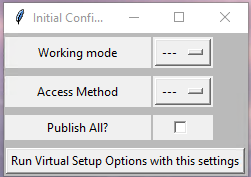
\includegraphics[width=0.7\linewidth]{proposed-work/bios-gui-initial-config}
	\caption{Menu to Select initial configuration for work}\label{fig:proposed-work-bios-gui-initial-config}
\end{figure}

\begin{figure}[!htbp]
	\centering
	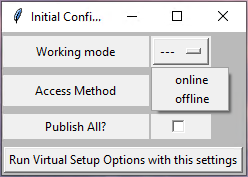
\includegraphics[width=0.7\linewidth]{proposed-work/bios-gui-initial-config-select-mode}
	\caption{Available work mode for the system: Online and Offline}\label{fig:proposed-work-bios-gui-initial-config-select-mode}
\end{figure}


Figure \ref{fig:proposed-work-bios-gui-acpi-knobs} shows the view that how an options in the module simulation is loaded.

\begin{table}
	\centering
	\renewcommand{\arraystretch}{2}
	\caption{Interpretation of buttons on Virtual Setup Page GUI}\label{table:interpretation-of-buttons-in-module}
	\begin{tabular}{l | p {6cm}}
		Button & Interpretation
		\\ \hline \hline
		Push Changes & Apply changes to system if online mode else apply changes to `bin` file
		\\ \hline View Changes & View saved changes in new window
		\\ \hline Exit & Exit the GUI
		\\ \hline Reload & Reload the GUI
		\\ \hline Discard Changes & Discard any change made, any value if modified are restored to current value
		\\ \hline Load Defaults & Restore to default values and revert any changes made
		\\ \hline 
	\end{tabular}
\end{table}

\begin{figure}[!htbp]
	\centering
	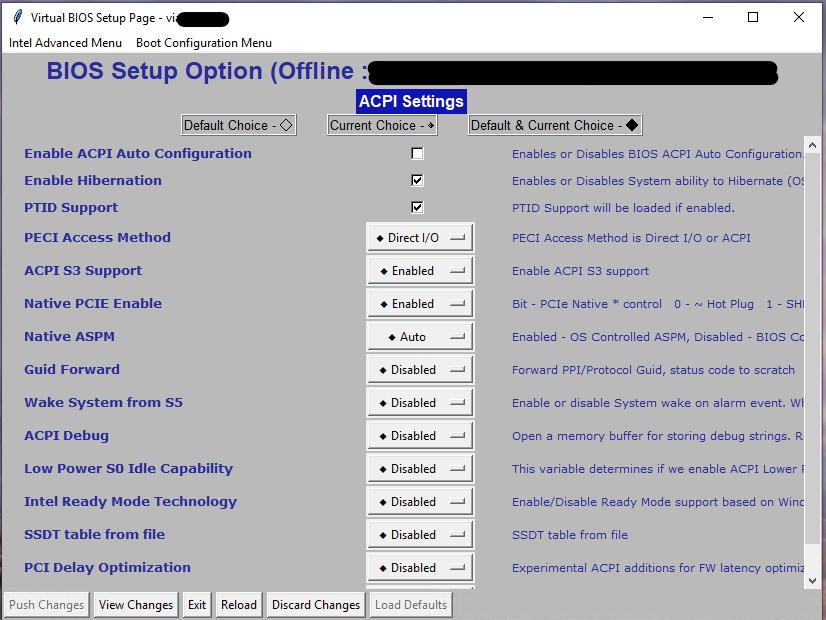
\includegraphics[width=0.8\linewidth]{proposed-work/bios-gui-acpi-knobs}
	\caption{Setup Options listed under ACPI Configurations}\label{fig:proposed-work-bios-gui-acpi-knobs}
\end{figure}

Table \ref{table:interpretation-of-buttons-in-module} describes the interpretation of each button action on specific condition as remarks if applicable


Navigation through the various BIOS pages can be done as shown in Figure \ref{fig:proposed-work-bios-gui-accessing-menu}.

\begin{figure}[!htbp]
	\centering
	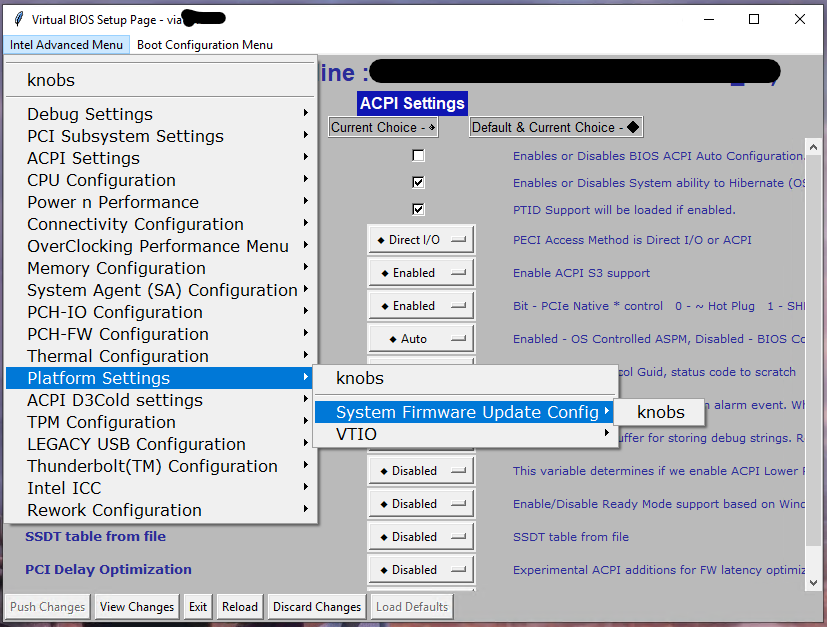
\includegraphics[width=0.8\linewidth]{proposed-work/bios-gui-accessing-menu}
	\caption{Navigating through BIOS setup page}\label{fig:proposed-work-bios-gui-accessing-menu}
\end{figure}

Figure \ref{fig:proposed-work-bios-gui-view-changes} displays list of changes made in setup options across any setup page and listed separately to compare with previous value, discard or apply the new values.

\begin{figure}[!htbp]
	\centering
	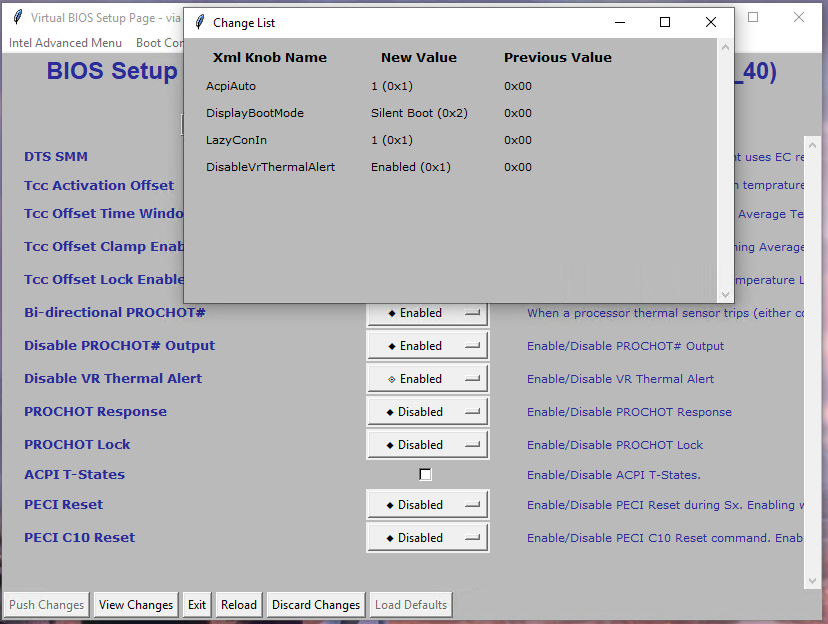
\includegraphics[width=\linewidth]{proposed-work/bios-gui-view-changes}
	\caption{Viewing all the changes made during current session}\label{fig:proposed-work-bios-gui-view-changes}
\end{figure}


\subsection{Processing Firmware individually}\label{subsection-processing-firmware}
To process apply the whole firmware changes individually for BIOS, signing is require to be performed for individual Firmware before stitching it to the BIOS binary in the valid structure.

\subsubsection{Primary Goals of the module}
\begin{itemize}
	\item Remove other Intellectual Property's dependency (\gls{ip} dependency) during firmware loading
	\item \gls{ip} Subsystem :
		\begin{itemize}
			\item Loader and Verifier
			\item \gls{ip} is always consumer
		\end{itemize}
	\item Signature verification using \gls{sha} hash algorithm and should be ease support for adding new algorithmic support as needed.
	\item Should support hardware based and software based verification support
	modifying memory requirements for given IP without impacting eco-system
	\item Prevent common security threats
	\item Allow easier OEM adoption and modification based on the respective design
	\item Reusability/Portability of design across many \gls{ip}s
	\item Generic design which supports any new IP integration
\end{itemize}

\begin{figure}[!htbp]
	\centering
	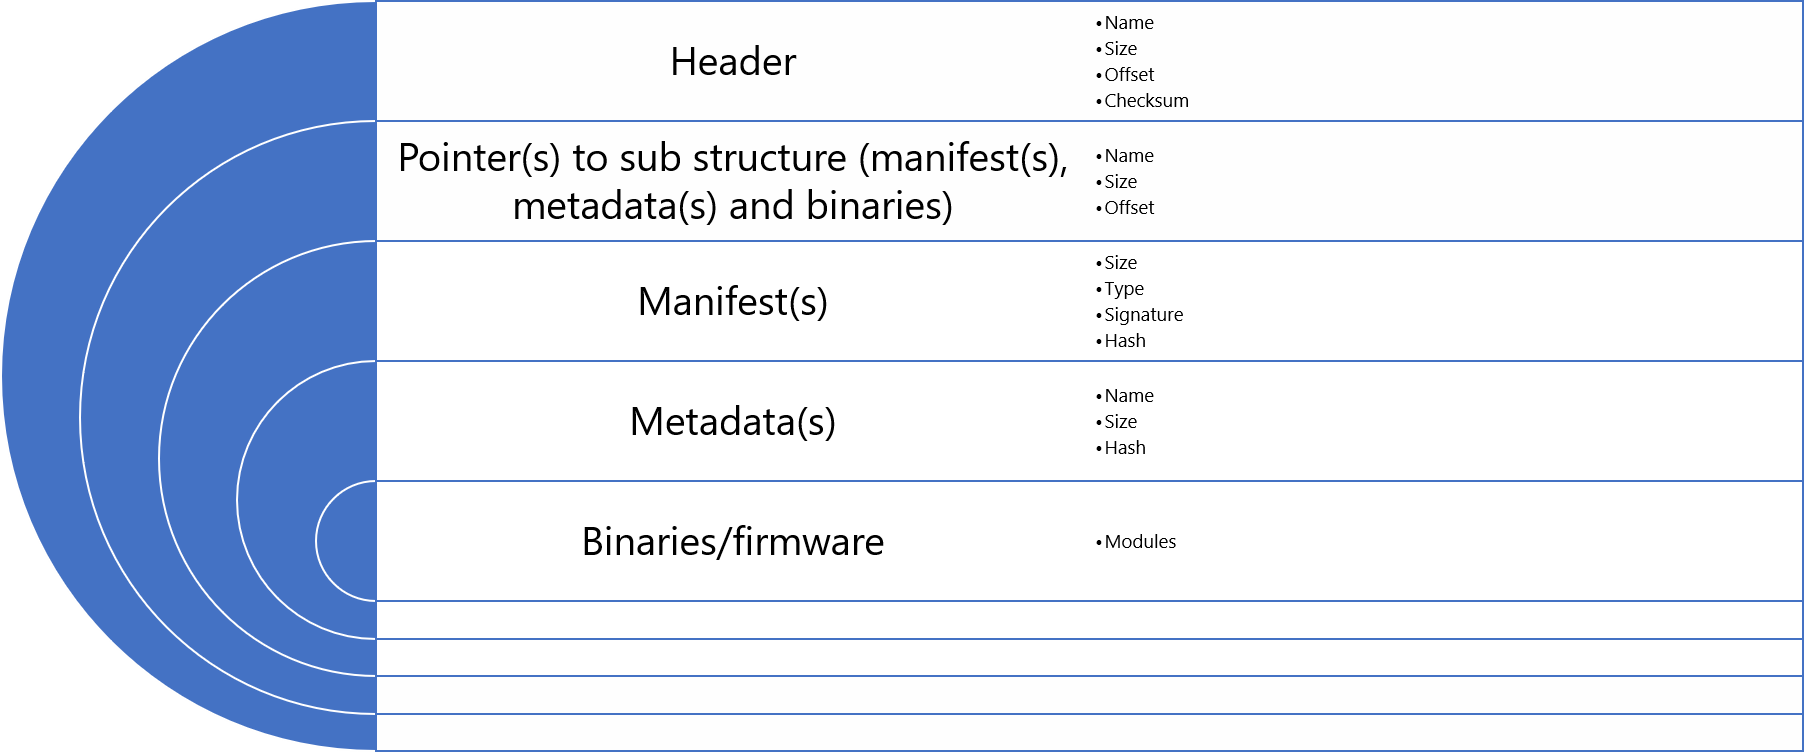
\includegraphics[width=\linewidth]{proposed-work/proposed-structure-firmware-signing}
	\caption{Proposed Structure for firmware signing}\label{fig:proposed-work-proposed-structure-firmware-signing}
\end{figure}
